Esse problema pode ser atacado considerando, em primeiro lugar, a matriz densidade inicial do sistema, dada por:

\begin{equation}
\rho(0) = \left[\begin{matrix}e^{- \Omega \left(\beta_{a} + \beta_{b}\right)} & 0 & 0 & 0\\0 & e^{\Omega \left(\beta_{a} - \beta_{b}\right)} & 0 & 0\\0 & 0 & e^{- \Omega \left(\beta_{a} - \beta_{b}\right)} & 0\\0 & 0 & 0 & e^{\Omega \left(\beta_{a} + \beta_{b}\right)}\end{matrix}\right]
\end{equation}

O Hamiltoniano, que descreverá a evolução do sistema, será dado por:

\begin{equation}
H =\left[\begin{matrix}\Omega & 0 & 0 & g\\0 & 0 & g & 0\\0 & g & 0 & 0\\g & 0 & 0 & - \Omega\end{matrix}\right]
\end{equation}

Esse Hamiltoniano pode ser diagonalizado, e sua forma diagonal fica:

\begin{equation}
H_d = \left[\begin{matrix}\sqrt{\Omega^{2} + g^{2}} & 0 & 0 & 0\\0 & - \sqrt{\Omega^{2} + g^{2}} & 0 & 0\\0 & 0 & g & 0\\0 & 0 & 0 & - g\end{matrix}\right]
\end{equation}

Isso pode ser feito com o auxílio da matriz $O$:

\begin{equation}
O = \left[\begin{matrix}\frac{\Omega + \sqrt{\Omega^{2} + g^{2}}}{\sqrt{g^{2} + \left(\Omega + \sqrt{\Omega^{2} + g^{2}}\right)^{2}}} & 0 & 0 & \frac{g}{\sqrt{g^{2} + \left(\Omega + \sqrt{\Omega^{2} + g^{2}}\right)^{2}}}\\\frac{\Omega - \sqrt{\Omega^{2} + g^{2}}}{\sqrt{g^{2} + \left(\Omega - \sqrt{\Omega^{2} + g^{2}}\right)^{2}}} & 0 & 0 & \frac{g}{\sqrt{g^{2} + \left(\Omega - \sqrt{\Omega^{2} + g^{2}}\right)^{2}}}\\0 & \frac{\sqrt{2}}{2} & \frac{\sqrt{2}}{2} & 0\\0 & \frac{\sqrt{2}}{2} & - \frac{\sqrt{2}}{2} & 0\end{matrix}\right]
\end{equation}

Teremos, então $O^{\textsc{T}} H_d O = H$ e $O^{\textsc{T}} O = \mathbb{1}$. Com o auxílio dessas matrizes, é possível construir a matriz de evolução temporal. Em primeiro lugar, sua forma diagonal será:

\begin{equation}
U_d = \left[\begin{matrix}e^{- i t \sqrt{\Omega^{2} + g^{2}}} & 0 & 0 & 0\\0 & e^{i t \sqrt{\Omega^{2} + g^{2}}} & 0 & 0\\0 & 0 & e^{- i g t} & 0\\0 & 0 & 0 & e^{i g t}\end{matrix}\right]
\end{equation}

Com o auxílio da matriz $O$, podemos trazer o operador de evolução para nossa representação original. Podemos então, utilizar esse operador e aplicar em nossa matriz densidade. Isso fornecerá a matriz densidade em qualquer instante do tempo:

\begin{equation}
\rho(t) = U^{\dagger} \rho U
\end{equation}

Utilizando então, a definição de valores esperados:

\begin{equation}
\langle A(t) \rangle = \Tr{\rho(t) \widehat{A}}
\end{equation}

Podemos, então obter o comportamento de diversos observáveis no tempo. Podemos observar na Figura \ref{g_grande} um exemplo. Podemos observar que há instantes no tempo em que boa parte da energia está retida na interação. Com a diminuição do parâmetro $g$, observamos o comportamento da Figura em \ref{g_pequeno}. É possível observar também que o sistema muda mais lentamente, consequência direta da diminuição da intensidade da componente de interação do Hamiltoniano.

\begin{figure}[!ht]
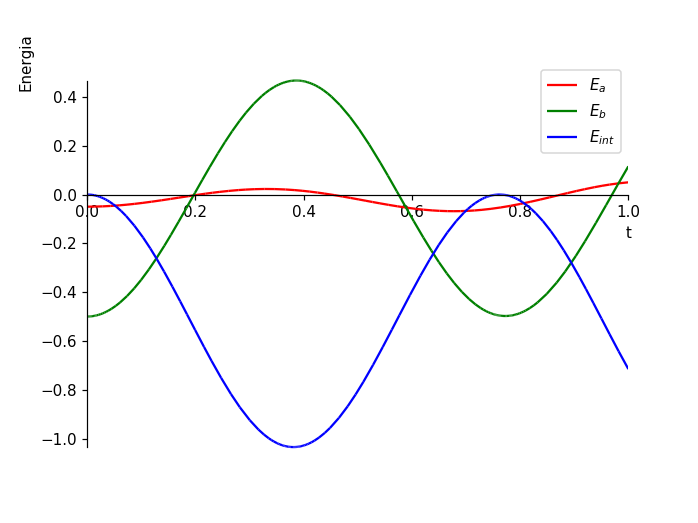
\includegraphics[scale=.4]{Content/g_grande.png}
\caption{Comportamento dos valores esperados de energia de pedaços do sistema. Os parâmetros escolhidos foram $\Omega = 1$, $g = 4$, $\beta_b=100$ e $\beta_a=0.1$.}
\label{g_grande}
\end{figure}

\begin{figure}[!ht]
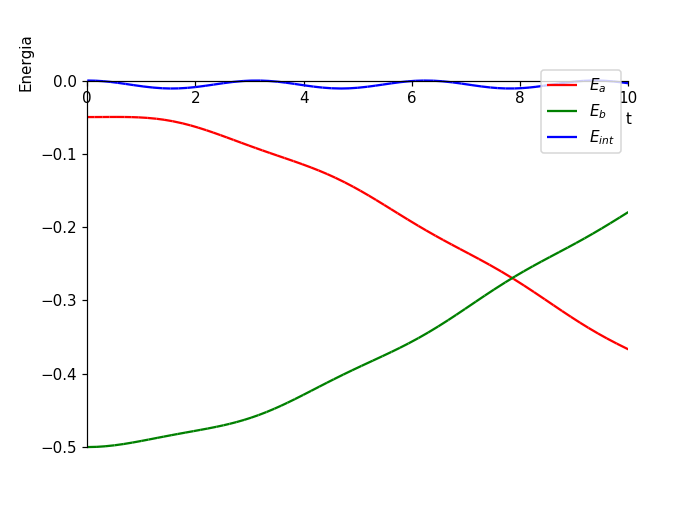
\includegraphics[scale=.4]{Content/g_pequeno.png}
\caption{Comportamento dos valores esperados de energia de pedaços do sistema. Os parâmetros escolhidos foram $\Omega = 1$, $g = 0.1$, $\beta_b=100$ e $\beta_a=0.1$.}
\label{g_pequeno}
\end{figure}

Quando inserimos \textbf{RWA}, o Hamiltoniano muda para:

\begin{equation}
H_{\text{RWA}} = \left[\begin{matrix}\Omega & 0 & 0 & 0\\0 & 0 & g & 0\\0 & g & 0 & 0\\0 & 0 & 0 & - \Omega\end{matrix}\right]
\end{equation}

Os autovalores são alterados, de maneira que o Hamiltoniano diagonal fica:

\begin{equation}
H_{d,\text{RWA}} = \left[\begin{matrix}\Omega & 0 & 0 & 0\\0 & - \Omega & 0 & 0\\0 & 0 & g & 0\\0 & 0 & 0 & - g\end{matrix}\right]
\end{equation}

Aplicando os métodos supramencionados, obtemos os comportamentos ilustrados pelas Figuras \ref{g_grande_rwa} e \ref{g_pequeno_rwa}. Podemos observar que a maior diferença foi no caso da Figura \ref{g_grande_rwa}. Nesse caso, para nenhum instante do tempo temos energia retida na interação. O que ilustra o fato de que a aproximação só é válida quando $\frac{g}{\Omega} \ll 1$.

\begin{figure}[!hb]
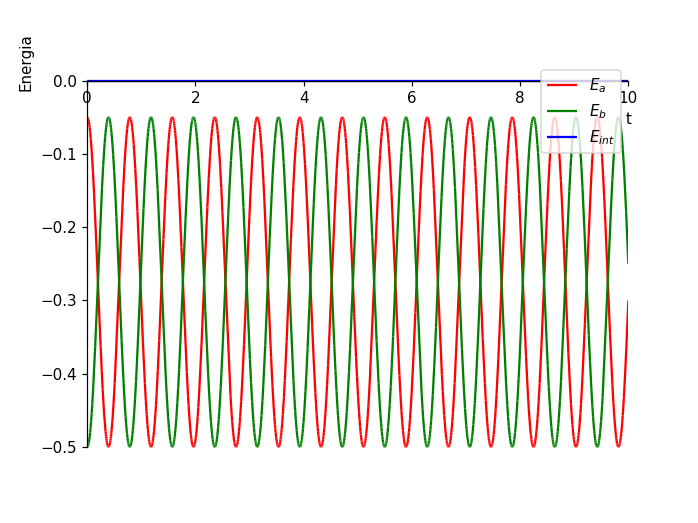
\includegraphics[scale=.4]{Content/g_grande_rwa.png}
\caption{Comportamento dos valores esperados de energia de pedaços do sistema. Os parâmetros escolhidos foram $\Omega = 1$, $g = 4$, $\beta_b=100$ e $\beta_a=0.1$. Nesse caso utilizamos a aproximação \textbf{RWA}.}
\label{g_grande_rwa}
\end{figure}

\begin{figure}[!ht]
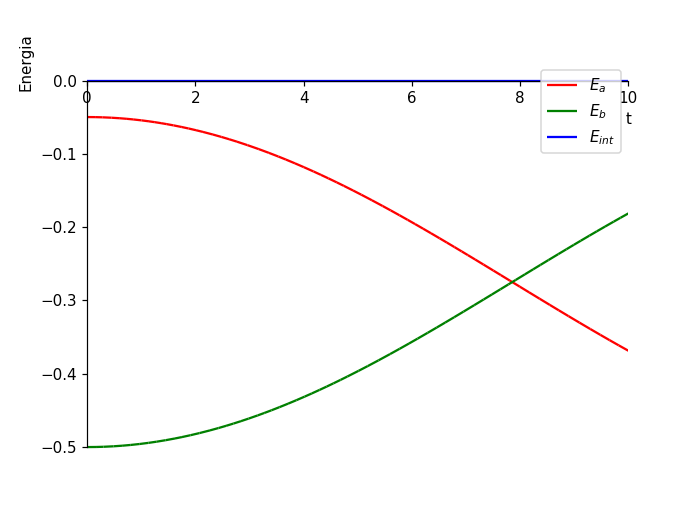
\includegraphics[scale=.4]{Content/g_pequeno_rwa.png}
\caption{Comportamento dos valores esperados de energia de pedaços do sistema. Os parâmetros escolhidos foram $\Omega = 1$, $g = 0.1$, $\beta_b=100$ e $\beta_a=0.1$. Nesse caso utilizamos a aproximação \textbf{RWA}.}
\label{g_pequeno_rwa}
\end{figure}
